\documentclass[11pt,a4paper,openany]{book}

% ---------- Encoding & Fonts ----------
\usepackage[T1]{fontenc}
\usepackage[utf8]{inputenc}
\usepackage{lmodern}
\usepackage{microtype}
\usepackage{textcomp}

% ---------- Geometry ----------
\usepackage[a4paper,margin=1.05in,headheight=14pt]{geometry}

% ---------- Math ----------
\usepackage{amsmath,amssymb,amsthm,mathtools}
\usepackage{bm}
\usepackage{nicefrac}
\usepackage{cancel}

% ---------- Graphics & Color ----------
\usepackage{graphicx}
\usepackage{xcolor}
\usepackage{tikz}
\usetikzlibrary{positioning,arrows.meta,shapes.geometric,fit,backgrounds,calc,decorations.pathmorphing}

% ---------- Tables ----------
\usepackage{booktabs}
\usepackage{array}
\usepackage{tabularx}
\usepackage{longtable}

% ---------- Lists & Misc ----------
\usepackage{enumitem}
\setlist{itemsep=2pt,topsep=3pt,parsep=1pt}
\usepackage{multicol}
\usepackage{epigraph}
\setlength\epigraphwidth{0.7\textwidth}

% ---------- Code listings ----------
\usepackage{listings}
\definecolor{codebg}{RGB}{248,248,248}
\definecolor{codekw}{RGB}{30,80,160}
\definecolor{codestr}{RGB}{160,40,40}
\definecolor{codecom}{RGB}{90,120,90}
\definecolor{coderule}{RGB}{200,200,200}
\lstset{
  basicstyle=\ttfamily\footnotesize,
  keywordstyle=\color{codekw}\bfseries,
  stringstyle=\color{codestr},
  commentstyle=\color{codecom}\itshape,
  backgroundcolor=\color{codebg},
  frame=single,
  rulecolor=\color{coderule},
  numbers=left,
  numberstyle=\tiny\color{gray},
  numbersep=8pt,
  breaklines=true,
  breakatwhitespace=true,
  showstringspaces=false,
  captionpos=b,
  xleftmargin=14pt,
  framexleftmargin=14pt,
}

% ---------- Boxes (theorems, definitions, pitfalls) ----------
\usepackage[most]{tcolorbox}
\tcbuselibrary{theorems,breakable,skins}

\definecolor{accent}{HTML}{1F3A93}
\definecolor{accent2}{HTML}{8E2DE2}
\definecolor{accent3}{HTML}{0A8754}
\definecolor{warn}{HTML}{B83227}
\definecolor{soft}{HTML}{F4F6FA}

\newtcbtheorem[number within=chapter]{defn}{Definition}
{enhanced,breakable,colback=soft,colframe=accent,boxrule=0.6pt,
 fonttitle=\bfseries\color{white},coltitle=white,
 attach boxed title to top left={xshift=8pt,yshift=-3pt},
 boxed title style={colback=accent,boxrule=0pt,sharp corners}}{def}

\newtcbtheorem[number within=chapter]{thm}{Theorem}
{enhanced,breakable,colback=soft,colframe=accent3,boxrule=0.6pt,
 fonttitle=\bfseries\color{white},coltitle=white,
 attach boxed title to top left={xshift=8pt,yshift=-3pt},
 boxed title style={colback=accent3,boxrule=0pt,sharp corners}}{thm}

\newtcolorbox{pitfall}[1]{enhanced,breakable,colback=red!4,
 colframe=warn,boxrule=0.6pt,title={\bfseries Pitfall: #1},
 fonttitle=\color{white},coltitle=white,
 attach boxed title to top left={xshift=8pt,yshift=-3pt},
 boxed title style={colback=warn,boxrule=0pt,sharp corners}}

\newtcolorbox{insight}[1]{enhanced,breakable,colback=accent2!5,
 colframe=accent2,boxrule=0.6pt,title={\bfseries Insight: #1},
 fonttitle=\color{white},coltitle=white,
 attach boxed title to top left={xshift=8pt,yshift=-3pt},
 boxed title style={colback=accent2,boxrule=0pt,sharp corners}}

\newtcolorbox{recipe}[1]{enhanced,breakable,colback=accent3!4,
 colframe=accent3,boxrule=0.6pt,title={\bfseries Recipe: #1},
 fonttitle=\color{white},coltitle=white,
 attach boxed title to top left={xshift=8pt,yshift=-3pt},
 boxed title style={colback=accent3,boxrule=0pt,sharp corners}}

% ---------- Headers / TOC ----------
\usepackage{fancyhdr}
\pagestyle{fancy}
\fancyhf{}
\renewcommand{\chaptermark}[1]{\markboth{\thechapter.\ #1}{}}
\renewcommand{\sectionmark}[1]{\markright{\thesection\ #1}{}}
\fancyhead[LE]{\small\nouppercase{\leftmark}}
\fancyhead[RO]{\small\nouppercase{\rightmark}}
\fancyfoot[LE,RO]{\thepage}
\fancyfoot[LO,RE]{\small\itshape SciML \& Dynamical Systems Bible}
\renewcommand{\headrulewidth}{0.4pt}

\usepackage[titles]{tocloft}
\renewcommand{\cftchapfont}{\bfseries\color{accent}}
\renewcommand{\cftchappagefont}{\bfseries\color{accent}}

% ---------- Chapter style ----------
\usepackage[Bjornstrup]{fncychap}

% ---------- Hyperref / cleveref ----------
\usepackage[hidelinks,bookmarksnumbered,bookmarksopen,colorlinks,
            linkcolor=accent,citecolor=accent3,urlcolor=accent2]{hyperref}
\usepackage[capitalize,noabbrev]{cleveref}

% ---------- Bibliography ----------
\usepackage[backend=biber,style=numeric-comp,sorting=none,maxbibnames=6,maxcitenames=2,giveninits=true]{biblatex}
\addbibresource{references.bib}

% ---------- Math operators / shortcuts ----------
\DeclareMathOperator*{\argmin}{arg\,min}
\DeclareMathOperator*{\argmax}{arg\,max}
\DeclareMathOperator{\E}{\mathbb{E}}
\DeclareMathOperator{\Var}{Var}
\DeclareMathOperator{\Cov}{Cov}
\DeclareMathOperator{\KL}{KL}
\DeclareMathOperator{\Tr}{Tr}
\DeclareMathOperator{\diag}{diag}
\DeclareMathOperator{\sgn}{sgn}
\newcommand{\R}{\mathbb{R}}
\newcommand{\N}{\mathbb{N}}
\newcommand{\C}{\mathbb{C}}
\newcommand{\Z}{\mathbb{Z}}
\newcommand{\Oh}{\mathcal{O}}
\newcommand{\Bop}{\mathcal{B}}
\newcommand{\T}{\mathsf{T}}
\newcommand{\dd}{\mathrm{d}}
\newcommand{\D}{\mathcal{D}}
\newcommand{\Lop}{\mathcal{L}}
\newcommand{\Nop}{\mathcal{N}}
\newcommand{\Gop}{\mathcal{G}}
\newcommand{\Hop}{\mathcal{H}}
\newcommand{\Kop}{\mathcal{K}}
\newcommand{\Pop}{\mathcal{P}}
\newcommand{\F}{\mathcal{F}}
\newcommand{\X}{\mathcal{X}}
\newcommand{\Y}{\mathcal{Y}}
\newcommand{\param}{\theta}

\title{\Huge\bfseries A Bible of Scientific Machine Learning\\[0.3em]
\Large\itshape Dynamical Systems, Operators, and the Frontier of\\
Physics-Aware Deep Learning}
\author{Compiled for Julian Chan\\\small PhD researcher, Astrophysics \& Machine Learning}
\date{\today}

\begin{document}

% =========================================================
\frontmatter

\begin{titlepage}
\centering
\vspace*{2cm}

\begin{tikzpicture}[remember picture,overlay]
  \fill[accent] ([yshift=-1.0cm]current page.north west) rectangle ([yshift=-1.6cm]current page.north east);
  \fill[accent2] ([yshift=-2.0cm]current page.north west) rectangle ([yshift=-2.06cm]current page.north east);
\end{tikzpicture}

\vspace{2.5cm}

{\Huge\bfseries\color{accent} A Bible of Scientific\\[0.25em] Machine Learning}\\[1.2em]
{\Large\itshape Dynamical Systems, Operators, and the Frontier\\[0.2em] of Physics-Aware Deep Learning}\\[3.5cm]

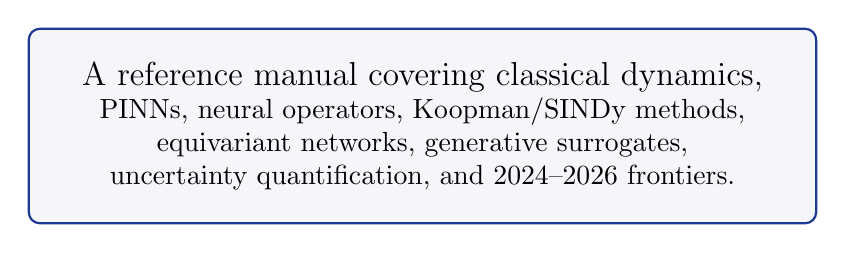
\begin{tikzpicture}
  \node[draw=accent,line width=0.8pt,rounded corners=4pt,inner sep=12pt,
        fill=soft,minimum width=10cm,align=center]
    {\large A reference manual covering classical dynamics,\\
     PINNs, neural operators, Koopman/SINDy methods,\\
     equivariant networks, generative surrogates,\\
     uncertainty quantification, and 2024--2026 frontiers.};
\end{tikzpicture}

\vfill
{\large Compiled for \textbf{Julian Chan}}\\[0.3em]
{\small PhD researcher --- Astrophysics \& Machine Learning}\\[0.3em]
{\small \today}
\end{titlepage}

\cleardoublepage
\thispagestyle{empty}
\vspace*{4cm}
\begin{center}
\itshape
\begin{minipage}{0.8\textwidth}
\centering
``All models are wrong, but some are useful.''\\[0.2em]
--- George E.\ P.\ Box\\[1em]
``It is the theory which decides what we can observe.''\\[0.2em]
--- Albert Einstein\\[1em]
``Mathematics is the art of giving the same name to different things.''\\[0.2em]
--- Henri Poincar\'e
\end{minipage}
\end{center}
\cleardoublepage

\chapter*{Preface}
\addcontentsline{toc}{chapter}{Preface}
\markboth{Preface}{Preface}

Scientific Machine Learning (SciML) is the discipline that fuses the
\emph{inductive bias of physics} with the \emph{expressive flexibility
of modern deep learning}. Where classical numerical analysis treats the
governing equations of nature as the primary object and data as a
secondary product, and where pure machine learning treats data as
primary and equations as optional, SciML insists on the dialogue
between the two. The result is a family of methods --- physics-informed
neural networks, neural operators, Koopman embeddings, universal
differential equations, equivariant networks, diffusion-based
surrogates, foundation models for physics --- that are reshaping how
scientists model complex dynamical systems.

\section*{Who this is for}
This document is written for advanced graduate students and researchers
working at the intersection of dynamical systems, numerical analysis,
and deep learning. It assumes familiarity with multivariable calculus,
linear algebra, ODE/PDE theory, and the basic apparatus of supervised
deep learning (backpropagation, optimisation, common architectures).

\section*{How to read it}
The book is structured as a reference. Part~I (Chapters~1--2) lays the
mathematical foundations of dynamical systems and classical
numerics. Part~II (Chapters~3--7) covers the core SciML toolkit. Part~III
(Chapters~8--11) addresses geometric, generative, and probabilistic
extensions. Part~IV (Chapters~12--13) surveys software, benchmarks,
and emerging trends through the 2024--2026 horizon. The appendix
(Chapter~14) collects functional analysis, automatic differentiation,
and stochastic calculus prerequisites.

Theorems, definitions, recipes, pitfalls, and insights are colour-coded
throughout to help the reader scan rapidly:

\begin{recipe}{Pseudocode and step-by-step procedures}
Practical workflows live in green recipe boxes.
\end{recipe}
\begin{insight}{Conceptual remarks}
Purple boxes flag conceptual subtleties or unifying perspectives.
\end{insight}
\begin{pitfall}{Things that go wrong}
Red boxes highlight failure modes that have caught practitioners.
\end{pitfall}

\section*{Notation}
We follow standard conventions: bold lowercase for vectors
($\bm{x}\in\R^d$), bold uppercase for matrices ($\bm{A}$), calligraphic
for operators and function spaces ($\mathcal{L},\mathcal{G},\mathcal{H}$).
Time is denoted $t$, spatial coordinates $\bm{x}$ or $\bm{\xi}$.
Neural network parameters are $\theta$. Probability density functions
are $p(\cdot)$. Expectations are $\E[\cdot]$. The differential
operator is $\partial$, the gradient $\nabla$, the Laplacian $\Delta$,
and the divergence $\nabla\cdot$.

\section*{Caveats}
SciML moves fast. Where possible we highlight \emph{stable principles}
rather than transient implementations. Citations point to canonical
references; the field's pace means new results may already supersede
specific benchmarks by the time of reading.


\tableofcontents
\cleardoublepage

% =========================================================
\mainmatter

\chapter{Foundations of Dynamical Systems}
\label{ch:foundations}

\epigraph{\itshape The whole of science is nothing more than a refinement of
everyday thinking.}{Albert Einstein}

\section{What is a dynamical system?}
A \emph{dynamical system} is a triple $(M,T,\Phi)$ where $M$ is a state
space (a manifold), $T$ is a time set (typically $\R$ or $\Z$), and
$\Phi:T\times M\to M$ is an evolution map satisfying the semi-group
axioms
\begin{align}
\Phi(0,\bm{x})&=\bm{x},\\
\Phi(t+s,\bm{x})&=\Phi(t,\Phi(s,\bm{x})).
\end{align}
Continuous-time systems are usually specified by an ODE
\begin{equation}
\dot{\bm{x}} = \bm{f}(\bm{x},t;\mu),\qquad \bm{x}(0)=\bm{x}_0,
\label{eq:ode}
\end{equation}
with parameter $\mu\in\R^p$. Discrete systems are given by a map
$\bm{x}_{k+1}=\bm{F}(\bm{x}_k)$. Spatially extended systems are modelled
by PDEs and become infinite-dimensional dynamical systems on
function spaces.

\begin{defn}{Flow and orbit}{flow}
The \emph{flow} of \cref{eq:ode} is the family of maps
$\{\Phi^t\}_{t\in\R}$ with $\Phi^t(\bm{x}_0)=\bm{x}(t)$. The
\emph{orbit} through $\bm{x}_0$ is the set
$\gamma(\bm{x}_0)=\{\Phi^t(\bm{x}_0):t\in\R\}$.
\end{defn}

\section{Linear systems and stability}
For the linear ODE $\dot{\bm{x}}=\bm{A}\bm{x}$ the solution is
$\bm{x}(t)=e^{t\bm{A}}\bm{x}_0$. The eigenvalues of $\bm{A}$ classify
the origin: stable node, unstable node, saddle, focus, centre. For
nonlinear systems, the \emph{Hartman--Grobman theorem} guarantees that,
near a hyperbolic fixed point, the flow is topologically conjugate to
its linearisation.

\begin{thm}{Lyapunov stability}{lyapunov}
Let $\bm{x}^\star$ be an equilibrium of \cref{eq:ode}. If there exists
a continuously differentiable function $V:\Omega\to\R$ on a neighbourhood
$\Omega\ni\bm{x}^\star$ with $V(\bm{x}^\star)=0$, $V(\bm{x})>0$ for
$\bm{x}\neq\bm{x}^\star$, and $\dot V(\bm{x})\le 0$ on $\Omega$, then
$\bm{x}^\star$ is Lyapunov stable. If $\dot V<0$ strictly, it is
asymptotically stable.
\end{thm}

\section{Nonlinear phenomena}
Nonlinearity introduces phenomena absent from linear theory:
\begin{itemize}
\item \textbf{Limit cycles:} isolated periodic orbits (Van der Pol).
\item \textbf{Bifurcations:} qualitative changes of phase portraits as
parameters vary --- saddle-node, transcritical, pitchfork, Hopf, period
doubling, homoclinic.
\item \textbf{Chaos:} sensitive dependence on initial conditions; the
maximal Lyapunov exponent
$\lambda_{\max}=\lim_{t\to\infty}\tfrac{1}{t}\log\|\delta\bm{x}(t)\|/\|\delta\bm{x}(0)\|$
is positive.
\item \textbf{Strange attractors:} fractal invariant sets attracting
nearby orbits (Lorenz, R\"ossler, Chua).
\end{itemize}

\begin{insight}{Why dynamics matters for ML}
Many learning algorithms are themselves dynamical systems: gradient
descent is an Euler discretisation of gradient flow $\dot\theta=-\nabla
L(\theta)$; momentum methods correspond to damped Hamiltonian
dynamics; sampling algorithms (Langevin, HMC) are stochastic flows on
parameter space. The mathematical machinery in this chapter is therefore
both the \emph{object} and the \emph{tool} of SciML.
\end{insight}

\section{Hamiltonian and Lagrangian mechanics}
Many physical systems possess a symplectic structure. Given a
configuration manifold $Q$ with coordinates $\bm{q}$ and conjugate
momenta $\bm{p}$, the \emph{Hamiltonian} $H(\bm{q},\bm{p},t)$ generates
flow via
\begin{equation}
\dot{\bm{q}}=\frac{\partial H}{\partial \bm{p}},\qquad
\dot{\bm{p}}=-\frac{\partial H}{\partial \bm{q}}.
\end{equation}
The 2-form $\omega=\dd\bm{q}\wedge\dd\bm{p}$ is preserved along the
flow. Equivalently, the Lagrangian $L(\bm{q},\dot{\bm{q}},t)=T-V$
satisfies the Euler--Lagrange equations
\begin{equation}
\frac{\dd}{\dd t}\frac{\partial L}{\partial \dot{\bm{q}}}-\frac{\partial L}{\partial \bm{q}}=0.
\end{equation}
Noether's theorem connects continuous symmetries to conserved
quantities --- a principle that motivates both equivariant neural
architectures (\cref{ch:equivariant}) and Hamiltonian/Lagrangian neural
networks (\cref{ch:nodes}).

\section{Partial differential equations}
A PDE is a relation
$\Nop[u](\bm{x},t)=0$ on a domain $\Omega\subset\R^d$, with boundary
conditions on $\partial\Omega$ and (for evolution problems) initial
conditions at $t=0$. Major classes:
\begin{itemize}
\item \textbf{Elliptic:} $-\Delta u=f$ (Poisson), steady-state.
\item \textbf{Parabolic:} $\partial_t u=\Delta u+f$ (heat), diffusive.
\item \textbf{Hyperbolic:} $\partial_t^2 u=c^2\Delta u$ (wave),
finite propagation speed.
\item \textbf{Conservation laws:} $\partial_t u+\nabla\cdot\bm{F}(u)=0$
(Burgers, Euler, Navier--Stokes).
\end{itemize}

Well-posedness in the sense of Hadamard requires existence,
uniqueness, and continuous dependence on data. For nonlinear hyperbolic
laws, \emph{weak} (entropy) solutions handle shock formation; we will
return to this when discussing PINN failure modes
(\cref{sec:pinn-failure}).

\section{Function spaces and the operator picture}
Solutions of PDEs live in function spaces (Sobolev, Bochner, etc.).
The map from problem data (coefficients, forcing, BCs, ICs) to solution
\begin{equation}
\Gop:\X\to\Y,\qquad a\mapsto u
\end{equation}
is the \emph{solution operator}. Most modern SciML --- especially
neural operators (\cref{ch:operators}) --- aims to learn $\Gop$
directly, rather than its values $u$ for fixed $a$.

\begin{recipe}{Picking the right viewpoint}
\begin{enumerate}
\item Single trajectory, fixed parameters: ODE/PDE \emph{solver}.
\item Family of trajectories, varying ICs: \emph{flow map} learning
(neural ODE, time-stepping operator).
\item Family of problem instances: \emph{solution operator} learning
(DeepONet, FNO).
\item Sparse data, unknown equation: \emph{system identification}
(SINDy, UDEs).
\end{enumerate}
\end{recipe}

\section{Stochastic dynamics}
When noise matters, replace the ODE by an SDE
\begin{equation}
\dd\bm{X}_t = \bm{f}(\bm{X}_t,t)\dd t + \bm{\sigma}(\bm{X}_t,t)\dd \bm{W}_t,
\end{equation}
with $\bm{W}_t$ a Wiener process. The Fokker--Planck equation governs
the density:
\begin{equation}
\partial_t p = -\nabla\!\cdot(\bm{f}p) + \tfrac{1}{2}\nabla\nabla:(\bm{\sigma}\bm{\sigma}^\T p).
\end{equation}
This connection between trajectories and densities is central to
\emph{score-based diffusion models} (\cref{ch:generative}), where the
reverse-time SDE is parameterised by a learned score
$\nabla\log p_t$.

\section{Inverse problems}
Many SciML applications are inverse: given observations
$\bm{y}=\Hop\bm{u}+\bm{\eta}$ of a state governed by a PDE, infer
parameters or initial conditions. Tikhonov regularisation, Bayesian
inference, and adjoint methods provide the classical scaffolding;
deep learning provides priors (deep image prior, score priors) and
amortised solvers.

\section{Summary}
Dynamical systems theory provides the language of states, flows,
stability, and conservation. Numerical analysis (\cref{ch:numerics})
provides tools to compute. Modern SciML threads neural networks
through both: as solvers, as surrogates, as identifiers, and as priors.

\chapter{Classical Numerical Methods}
\label{ch:numerics}

\epigraph{\itshape A good approximation is one that holds together for a
while, and then breaks in a way you understand.}{Folklore in numerical
analysis}

A SciML practitioner cannot escape numerical analysis: it furnishes
the training data, the baselines, and the inductive biases for many
neural-network methods.

\section{Time integration of ODEs}
Given $\dot{\bm{x}}=\bm{f}(\bm{x},t)$, denote the time step $h$.

\subsection{Explicit Runge--Kutta}
The classical $s$-stage RK scheme is
\begin{equation}
\bm{k}_i = \bm{f}\!\left(\bm{x}_n + h\sum_{j=1}^{i-1}a_{ij}\bm{k}_j,\; t_n+c_ih\right),\quad
\bm{x}_{n+1}=\bm{x}_n+h\sum_{i=1}^s b_i\bm{k}_i.
\end{equation}
RK4 ($s=4$) achieves order four with the well-known Butcher tableau.
Adaptive Dormand--Prince (DP5) embeds an order-4 estimator inside an
order-5 step for error control.

\subsection{Implicit and stiff solvers}
Stiff systems --- where the spectrum of the Jacobian spans many orders
of magnitude --- demand implicit methods. Backward differentiation
formulas (BDF), implicit RK (Radau, SDIRK), and Rosenbrock methods are
standard. The cost is a (possibly nonlinear) solve at each step.

\begin{insight}{Why ``stiff'' bites neural ODEs}
Neural ODEs use \emph{black-box} adaptive solvers and back-propagate
through them. When the learned dynamics become stiff, solver step
counts (and wall time) explode. Mitigations include semi-implicit
adjoints, regularising stiffness, or restricting parameterisations
(\cref{ch:nodes}).
\end{insight}

\subsection{Symplectic integrators}
For Hamiltonian systems, preserving $\omega$ matters more than local
order. \emph{St\"ormer--Verlet} and higher-order \emph{Yoshida}
splittings have bounded energy error over exponentially long times --
critical for n-body astrophysics.

\begin{recipe}{Choosing a time integrator}
\begin{enumerate}
\item Non-stiff, non-conservative: RK4, DP5, Tsit5.
\item Stiff: BDF, Radau IIA, Rosenbrock--Wanner.
\item Hamiltonian / long-horizon energy fidelity: Verlet, Yoshida-4.
\item Stochastic: Euler--Maruyama (order $\tfrac12$), Milstein
(order $1$), stochastic Runge--Kutta.
\end{enumerate}
\end{recipe}

\section{Spatial discretisation of PDEs}
\subsection{Finite differences (FD)}
Replace derivatives by stencils on a uniform grid:
$\partial_x u_i \approx (u_{i+1}-u_{i-1})/(2h)$. Easy to implement,
limited geometric flexibility, suffer at sharp gradients without
upwinding or limiters.

\subsection{Finite volumes (FV)}
Integrate conservation laws over control volumes; fluxes at faces are
reconstructed via Godunov / Roe / HLLC solvers. Native handling of
shocks and discrete conservation. Backbone of CFD codes.

\subsection{Finite elements (FE)}
Project the weak form $\int_\Omega(\Lop u)v\,\dd\Omega=\int_\Omega
fv\,\dd\Omega$ onto a finite-dimensional basis $\{\phi_j\}$.
Galerkin / Petrov--Galerkin / DG variants. Excellent on complex
geometries.

\subsection{Spectral methods}
Expand $u(\bm{x})=\sum_k \hat u_k\phi_k(\bm{x})$ in a global basis
(Fourier on tori, Chebyshev on intervals). Exponential convergence
for analytic solutions; foundational for Fourier neural operators
(\cref{sec:fno}).

\subsection{Mesh-free / particle methods}
Smoothed particle hydrodynamics (SPH), radial basis functions (RBF),
and reproducing kernel particle methods. Neural networks themselves can
be viewed as a mesh-free basis.

\section{Linear algebra and Krylov methods}
Most PDE discretisations reduce to large sparse linear systems
$\bm{A}\bm{u}=\bm{b}$. Conjugate gradient (CG), GMRES, BiCGStab, and
multigrid are workhorses. Preconditioning ($\bm{M}^{-1}\bm{A}\bm{u}=
\bm{M}^{-1}\bm{b}$) is often the difference between a usable and
unusable method.

\section{Adjoint and sensitivity analysis}
For gradient-based learning of physical parameters, the
\emph{continuous adjoint} computes
$\dd L/\dd\mu$ at cost independent of $\dim\mu$ via a backward ODE:
\begin{equation}
\dot{\bm{\lambda}} = -\bm{\lambda}^\T \frac{\partial \bm{f}}{\partial \bm{x}} - \frac{\partial \ell}{\partial \bm{x}},\qquad
\frac{\dd L}{\dd \mu} = \int_0^T \bm{\lambda}^\T \frac{\partial \bm{f}}{\partial \mu}\,\dd t.
\end{equation}
The discrete adjoint differentiates the solver itself; both are special
cases of automatic differentiation (Appendix~A).

\section{Stability, consistency, convergence}
The Lax equivalence theorem ties these together for linear problems:
\emph{a consistent finite-difference scheme is convergent if and only
if it is stable}. The CFL condition $|c|h_t\le h_x$ for advection,
the stiffness-driven step restriction for explicit parabolic
schemes, and the von Neumann amplification analysis are all canonical.
These constraints transfer almost verbatim to neural-network surrogates
that mimic explicit time-stepping.

\begin{pitfall}{Surrogate ``solvers'' that violate CFL}
A learned time-stepper trained on $\Delta t$ slightly larger than the
finest physical time scale may appear accurate in-distribution but
diverge catastrophically when rolled out --- exactly the failure mode
of an unstable explicit scheme. \emph{Train-time rollouts} or
implicit-style architectures help.
\end{pitfall}

\section{Reduced-order models (ROMs)}
For high-dimensional systems, project onto a low-dimensional subspace.
Proper Orthogonal Decomposition (POD) builds modes from snapshots via
SVD. Galerkin or Petrov--Galerkin projection yields a small ODE on the
modes. ROMs are often the bridge between full-order numerics and
neural-operator surrogates --- and provide Koopman/DMD with their data
(\cref{ch:operator-theoretic}).

\section{Summary}
Classical numerics gives us a vocabulary --- consistency, stability,
order, conservation, symplecticity --- that survives intact in modern
SciML, even when the basis functions are replaced by neural
networks. The interesting question is not whether to abandon classical
methods, but \emph{which of their structural properties to preserve}
inside a learned model.

\chapter{Neural ODEs, CDEs, and SDEs}
\label{ch:nodes}

\epigraph{\itshape A residual block is a discrete Euler step. Take the
limit and you have an ODE.}{Chen, Rubanova, Bettencourt, Duvenaud (2018)}

\section{From ResNets to Neural ODEs}
A residual block computes
$\bm{h}_{n+1}=\bm{h}_n+\bm{f}_\theta(\bm{h}_n)$. Treating depth as time
and taking $\Delta t\to 0$ gives the \emph{neural ODE}~\cite{chen2018neuralode}:
\begin{equation}
\frac{\dd \bm{h}(t)}{\dd t}=\bm{f}_\theta(\bm{h}(t),t),\qquad
\bm{h}(0)=\bm{x}.
\end{equation}
The ``forward pass'' is an ODE solve from $0$ to $T$. Memory cost is
$\Oh(1)$ in the number of steps because gradients are computed by
solving a backward adjoint ODE rather than storing intermediate states.

\subsection{Adjoint method}
Define the loss $L(\bm{h}(T))$. Introduce the adjoint
$\bm{a}(t)=\partial L/\partial \bm{h}(t)$, which satisfies
\begin{equation}
\frac{\dd \bm{a}(t)}{\dd t}=-\bm{a}(t)^\T \frac{\partial \bm{f}_\theta}{\partial \bm{h}}.
\end{equation}
The parameter gradient is
$\dd L/\dd\theta=-\int_0^T \bm{a}(t)^\T (\partial \bm{f}_\theta/\partial\theta)\,\dd t$.
This is the continuous-time analogue of backpropagation.

\begin{pitfall}{Adjoint instability}
The continuous adjoint can be numerically inaccurate when the forward
solver uses adaptive step control or interpolated dense output. The
\emph{interpolated} or \emph{checkpointed} adjoint, and JAX/PyTorch
\texttt{torchdiffeq} backsolve, mitigate this. For chaotic systems,
adjoints diverge along Lyapunov directions; consider shadowing /
ensemble adjoints.
\end{pitfall}

\section{Variants and architectures}
\paragraph{Augmented neural ODEs}
The flow of an ODE is a homeomorphism, so a neural ODE cannot represent
maps that change topology. Augmenting the state with extra dimensions
$\bm{a}(0)=\bm{0}$ restores expressivity~\cite{dupont2019anode}.

\paragraph{Latent ODEs and continuous normalising flows.}
For irregular time series and density estimation, model dynamics in a
latent space and decode~\cite{rubanova2019latentode}. Continuous
normalising flows (CNFs) use the instantaneous change-of-variables
formula
$\dd\log p/\dd t=-\Tr(\partial \bm{f}/\partial \bm{h})$ to evaluate
likelihoods.

\paragraph{Neural CDEs.}
For irregular time series, treat the data path $\bm{X}(t)$ as a
control and integrate
$\dd\bm{h}(t)=\bm{f}_\theta(\bm{h}(t))\,\dd\bm{X}(t)$ in the sense of
controlled differential equations~\cite{kidger2020ncde}.

\paragraph{Neural SDEs.}
Add Brownian motion: $\dd\bm{h}=\bm{f}_\theta\,\dd t+\bm{\sigma}_\theta\,\dd\bm{W}_t$.
Trainable via Wasserstein matching, KL with reference SDE, or score-matching;
foundational for generative diffusion (\cref{ch:generative}).

\section{Hamiltonian and Lagrangian neural networks}
Architectural priors that respect mechanics:
\begin{itemize}
\item \textbf{HNN}~\cite{greydanus2019hnn}: parameterise $H_\theta(\bm{q},\bm{p})$;
integrate $\dot{\bm{q}}=\partial_{\bm{p}}H_\theta$,
$\dot{\bm{p}}=-\partial_{\bm{q}}H_\theta$.
\item \textbf{LNN}~\cite{cranmer2020lnn}: parameterise $L_\theta(\bm{q},\dot{\bm{q}})$
and impose Euler--Lagrange equations.
\item \textbf{Symplectic ODE-Net, Constrained HNN}: enforce constraints
and conservation explicitly.
\end{itemize}
These networks generalise far beyond their training horizon precisely
because they encode the right invariant.

\section{ODE-based deep generative models}
\subsection{Continuous normalising flows (CNF)}
Train $\bm{f}_\theta$ so that the pushforward of a base density
matches the data density:
\begin{equation}
\log p_\theta(\bm{x})=\log p_0(\bm{h}(0)) - \int_0^T \nabla\!\cdot\bm{f}_\theta(\bm{h}(t),t)\,\dd t.
\end{equation}
\subsection{FFJORD and Hutchinson trace estimators}
Replace the exact trace by a Hutchinson estimator
$\Tr(\bm{J})\approx \E_{\bm{\epsilon}\sim\mathcal{N}}[\bm{\epsilon}^\T\bm{J}\bm{\epsilon}]$ for tractable training.

\subsection{Flow matching and stochastic interpolants}
Recent advances~\cite{lipman2023flowmatching,albergo2023interpolants}
train CNFs by regressing onto a target velocity field defined by a
prescribed interpolation between base and data distributions, avoiding
expensive ODE simulation during training. Discussed at length in
\cref{ch:generative}.

\section{Practical training tips}
\begin{recipe}{Training a neural ODE end-to-end}
\begin{enumerate}
\item Normalise inputs/outputs; centre time near zero.
\item Start with a permissive solver (Tsit5, atol/rtol $10^{-3}$) and
tighten as training progresses.
\item Use the \emph{checkpointed adjoint} for long horizons; the
\emph{recursive checkpoint} for memory.
\item Add Jacobian/Frobenius penalties to discourage stiffness.
\item Curriculum on $T$: train on short windows, extend gradually.
\end{enumerate}
\end{recipe}

\section{Where neural ODEs shine and where they struggle}
\textbf{Strengths:} natural for irregular time series, continuous-depth
generative modelling, mechanistic priors via HNN/LNN, smooth and
invertible models.\\
\textbf{Weaknesses:} high wall-clock cost from solver calls;
representation limited to homeomorphisms (without augmentation);
delicate adjoint behaviour on stiff or chaotic dynamics.

\begin{insight}{Neural ODE = parametric differential equation}
The most productive way to think about neural ODEs is not as a deep
network whose depth is continuous, but as a \emph{parametric ODE family
fitted to data}. This perspective unifies them with Universal
Differential Equations (\cref{ch:hybrid-ude}), system identification
(\cref{ch:operator-theoretic}), and operator learning
(\cref{ch:operators}).
\end{insight}

\chapter{Physics-Informed Neural Networks}
\label{ch:pinns}

\epigraph{\itshape A PINN is a neural network whose loss function is a
PDE.}{Raissi, Perdikaris, Karniadakis (2019)}

\section{Formulation}
Consider a PDE on $\Omega\times[0,T]$:
\begin{align}
\Nop[u](\bm{x},t)&=0 \quad \text{in } \Omega\times(0,T],\\
\Bop[u](\bm{x},t)&=g(\bm{x},t) \quad \text{on } \partial\Omega\times[0,T],\\
u(\bm{x},0)&=u_0(\bm{x}) \quad \text{in } \Omega.
\end{align}
A PINN parameterises $u\approx u_\theta:\R^{d+1}\to\R^k$ as a multilayer
perceptron and minimises a composite loss~\cite{raissi2019pinn}
\begin{equation}
\Lop(\theta) = w_r\Lop_r + w_b\Lop_b + w_0\Lop_0 + w_d\Lop_d,
\end{equation}
where
\begin{align}
\Lop_r &=\frac{1}{N_r}\sum_i \big|\Nop[u_\theta](\bm{x}_i,t_i)\big|^2,\\
\Lop_b &=\frac{1}{N_b}\sum_i \big|\Bop[u_\theta]-g\big|^2,\\
\Lop_0 &=\frac{1}{N_0}\sum_i \big|u_\theta(\bm{x}_i,0)-u_0\big|^2,\\
\Lop_d &=\frac{1}{N_d}\sum_i \big|u_\theta(\bm{x}_i,t_i)-u_i^{\text{obs}}\big|^2.
\end{align}
Derivatives appearing in $\Nop$ are obtained by automatic
differentiation through the network.

\section{Why it works (when it works)}
The PINN loss imposes the strong-form PDE on a finite set of
\emph{collocation points}. With sufficiently expressive $u_\theta$ and
adequate optimisation, $u_\theta$ approaches a strong solution. The
formulation is mesh-free, accommodates irregular geometries, and
unifies forward and inverse problems --- inverse coefficients become
trainable parameters.

\section{Variants}
\paragraph{XPINN / cPINN.}
Domain decomposition: separate networks per subdomain stitched together
by interface losses, enabling parallelism and capture of localised
features~\cite{jagtap2020xpinn}.

\paragraph{hp-VPINN.}
Use the variational (weak) form with test functions, integrating by
parts to reduce derivative orders --- helpful when solutions have low
regularity.

\paragraph{Causal PINN.}
Re-weight the time-domain residual to enforce that the loss at later
times is small only \emph{after} earlier times converge, avoiding
non-causal solutions to time-evolution PDEs~\cite{wang2022causal}.

\paragraph{NTK-based PINN.}
The neural tangent kernel reveals spectral bias in PINN training:
high-frequency residual modes converge slowly. Re-weighting based on
the NTK eigenvalues fixes the imbalance~\cite{wang2022ntkpinn}.

\paragraph{Self-adaptive / SA-PINN.}
Per-point trainable weights $\lambda_i$ adversarially upweight hard
collocation points~\cite{mcclenny2023sapinn}.

\paragraph{PINN-LS, gPINN, PIELM.}
Least-squares formulations, gradient-enhanced PINNs, and physics-informed
extreme learning machines trade off flexibility for speed.

\section{Failure modes}
\label{sec:pinn-failure}

PINNs are notoriously brittle. Documented failure modes include:
\begin{enumerate}
\item \textbf{Spectral bias} towards low frequencies; sharp gradients
and shock fronts under-resolved.
\item \textbf{Multi-objective imbalance}: residual, boundary, and data
losses conflict; gradient pathologies emerge.
\item \textbf{Stiffness in time}: optimiser converges to spurious steady
states matching the residual at $t=0$ but not propagating.
\item \textbf{Non-convex landscapes}: local minima where residual is
small but solution is wrong.
\item \textbf{Floating-point precision}: a 2025 result shows many
``failure modes'' disappear when training is performed in
\textsf{float64} rather than \textsf{float32}, because the L-BFGS
convergence test is otherwise triggered prematurely~\cite{rethinking2025pinn}.
\end{enumerate}

\begin{pitfall}{The ``trivial solution'' trap}
For homogeneous PDEs with zero forcing and inadequate boundary loss
weighting, a PINN can converge to $u_\theta\equiv 0$. Always sanity-check
the solution magnitude and inspect residual histograms by region.
\end{pitfall}

\subsection{Mitigations}
\begin{recipe}{Hardening a PINN}
\begin{enumerate}
\item Use \textsf{float64}; verify L-BFGS convergence flags.
\item Adaptive collocation: resample where residual is large (RAR,
RAD).
\item Loss balancing: NTK weights, gradient-norm balancing,
SoftAdapt, ReLoBRaLo.
\item Hard-constrain BCs/ICs by output transforms
$u_\theta(\bm{x},t) = u_0(\bm{x}) + t\,\bm{N}_\theta$.
\item Causal time-marching: train on expanding time windows.
\item Fourier features / SIREN activations to combat spectral bias.
\item Exact gradient computation; avoid \texttt{create\_graph=True}
pitfalls in PyTorch.
\end{enumerate}
\end{recipe}

\section{Inverse problems with PINNs}
PINNs shine in data-assimilation regimes where partial measurements
constrain unknown coefficients $\mu$ in $\Nop_\mu$. Joint optimisation
of $(\theta,\mu)$ gives forward + inverse for free. This is why PINNs
are popular in subsurface flow, biomechanics, and astrophysical fluid
inference.

\section{Theoretical guarantees}
Universal approximation extends to PINNs under mild regularity, but
\emph{trainability} is the binding constraint. Recent work bounds the
generalisation error in terms of the residual loss, neural tangent
kernel conditioning, and quadrature error of the collocation
sampling~\cite{wang2022ntkpinn,deryck2024pinns}.

\section{When to choose a PINN over alternatives}
\begin{insight}{PINNs vs. neural operators vs. classical solvers}
\begin{itemize}
\item Single problem instance, smooth solution, sparse data, want
mesh-free + inverse parameters: \emph{PINN}.
\item Many problem instances, repeated queries: \emph{neural operator}
(\cref{ch:operators}).
\item One-shot accuracy, complex geometry, no parameter unknowns:
classical FE/FV solver.
\item Stiff multiscale + partial data: \emph{universal differential
equations} (\cref{ch:hybrid-ude}).
\end{itemize}
\end{insight}

\section{Code skeleton (JAX)}
\begin{lstlisting}[language=Python,caption={Minimal PINN for 1D Burgers},label=lst:pinn]
import jax, jax.numpy as jnp, optax
from flax import linen as nn

class MLP(nn.Module):
    feats: tuple = (64,)*5
    @nn.compact
    def __call__(self, x):
        for f in self.feats:
            x = nn.tanh(nn.Dense(f)(x))
        return nn.Dense(1)(x)

def u_fn(params, x, t):
    return model.apply(params, jnp.stack([x, t]))[0]

def residual(params, x, t, nu=0.01/jnp.pi):
    u   = u_fn(params, x, t)
    u_t = jax.grad(u_fn, argnums=2)(params, x, t)
    u_x = jax.grad(u_fn, argnums=1)(params, x, t)
    u_xx= jax.grad(lambda p,x,t: jax.grad(u_fn,argnums=1)(p,x,t),argnums=1)(params,x,t)
    return u_t + u*u_x - nu*u_xx
\end{lstlisting}

\section{Summary}
PINNs remain a swiss-army knife when the equation is known, geometry is
awkward, and data is scarce. Their reputation for fragility is partly
fair and partly due to under-engineered training. With float64,
adaptive sampling, balanced losses, and causal training, vanilla PINNs
solve a remarkable range of problems --- a fact that the literature has
recently re-affirmed~\cite{rethinking2025pinn}.

\chapter{Neural Operators}
\label{ch:operators}

\epigraph{\itshape Operator learning is to function approximation what
calculus is to arithmetic.}{Anandkumar, Stuart and collaborators}

\section{Solution operators}
The forward map of a parameterised PDE family is an operator
\begin{equation}
\Gop : a\in\mathcal{A} \;\longmapsto\; u\in\mathcal{U},
\end{equation}
between Banach spaces of functions. Where a PINN learns one $u$, a
\emph{neural operator} learns $\Gop$. Once trained, evaluating $\Gop$
on a new $a$ is a forward pass --- orders of magnitude faster than a
fresh PDE solve.

\section{DeepONet}
DeepONet~\cite{lu2021deeponet} factorises the operator into branch and
trunk networks:
\begin{equation}
\Gop[a](\bm{y}) \approx \sum_{k=1}^p b_k(a(\bm{x}_1),\dots,a(\bm{x}_m))\,t_k(\bm{y}),
\end{equation}
where the \emph{branch} $\bm{b}$ encodes the input function (sampled at
sensors $\bm{x}_i$) and the \emph{trunk} $\bm{t}$ encodes the query
point $\bm{y}$. The architecture is justified by a universal
approximation theorem for nonlinear continuous operators (Chen \& Chen
1995). Variants: POD-DeepONet, multiple-input DeepONet, physics-informed
DeepONet.

\section{Fourier Neural Operator (FNO)}
\label{sec:fno}
FNO~\cite{li2021fno} parameterises the operator as a sequence of layers
\begin{equation}
v_{\ell+1}(\bm{x}) = \sigma\!\left(\bm{W}v_\ell(\bm{x}) + \F^{-1}(\bm{R}_\ell\cdot \F v_\ell)(\bm{x})\right),
\end{equation}
where $\F$ is the Fourier transform and $\bm{R}_\ell$ is a learned
truncated convolution kernel acting on the lowest $K$ modes. Key
properties:
\begin{itemize}
\item Discretisation invariance: trained on one resolution, queried at
another (with caveats).
\item Quasi-linear cost via FFT: $\Oh(N\log N)$ per layer.
\item Strong empirical performance on smooth periodic problems.
\end{itemize}

\subsection{Variants of FNO}
\paragraph{Geo-FNO, Factorised FNO, Tensor-FNO.}
Handle non-rectangular domains by warping geometries; factorise modes
across dimensions; tensor-decompose the kernel.
\paragraph{U-FNO, U-Net FNO.}
Combine FNO with U-Net hierarchy for multiscale features.
\paragraph{Spherical FNO}~\cite{bonev2023sfno}.
Replace FFT with spherical harmonic transforms; used for
state-of-the-art global weather emulators (FourCastNet, GraphCast
hybrids).
\paragraph{Adaptive FNO and AFNO.}
Adapt mode truncation per token, used inside vision transformers.

\begin{pitfall}{FNO discretisation invariance, with asterisks}
Out-of-distribution behaviour at resolutions far from training is
dataset-dependent. Aliasing, periodic-padding artefacts, and limited
mode budgets can all break the ``train once, query anywhere'' promise.
Always benchmark on multiple resolutions.
\end{pitfall}

\section{Graph Neural Operators}
For unstructured meshes, GNOs~\cite{li2020gno,brandstetter2022mpneural}
parameterise an integral operator
\begin{equation}
v_{\ell+1}(\bm{x}) = \sigma\!\left(\bm{W}v_\ell(\bm{x}) + \int_{B_r(\bm{x})}\kappa_\theta(\bm{x},\bm{y})v_\ell(\bm{y})\,\dd\bm{y}\right)
\end{equation}
via message passing on a graph built from the mesh. MeshGraphNet,
GNN-FNO hybrids, and the message-passing PDE solver belong to this
family.

\section{Transformer-based operators}
Transformers naturally handle variable-length, irregular inputs. Recent
high-impact systems include:
\begin{itemize}
\item \textbf{GNOT, OFormer, GAOT}: cross-attention between query
points and conditioning.
\item \textbf{Transolver}: token-mixing in physical space with attention
across slices.
\item \textbf{DPOT, MPP, Poseidon}: transformer-based foundation models
(\cref{ch:emerging}).
\end{itemize}

\paragraph{Poseidon}~\cite{herde2024poseidon} is a multiscale operator
transformer pretrained on a heterogeneous mix of PDE families with
\emph{time-conditioned layer norms} and a semi-group training loss; it
demonstrates strong few-shot transfer to new PDEs.

\section{Discretisation invariance: theory}
A defining requirement of a \emph{neural operator} (vs.\ a
discretisation-tied surrogate) is that it is well-defined as a map
between function spaces, with finite-dimensional implementations
recovered as projections~\cite{kovachki2023neural}. Universal
approximation theorems exist for FNO, DeepONet, and graph operators
under appropriate compactness assumptions.

\section{Training data}
\begin{recipe}{Building a neural-operator dataset}
\begin{enumerate}
\item Define the PDE family by sampling parameters/coefficients/ICs from
a distribution that covers downstream use.
\item Solve with a high-fidelity classical solver; store inputs $a_i$
and solutions $u_i$ at multiple resolutions / time steps.
\item Decide loss: relative $L^2$, $H^1$, or task-specific energy norms.
\item For time-dependent operators, choose autoregressive (next-step) or
direct (input-to-final) framing; combine with rollout regularisation.
\item Augment with symmetries (translation, rotation, reflection) when
the PDE allows.
\end{enumerate}
\end{recipe}

\section{Beyond pure data: physics-informed operators}
Add residual losses on the operator output:
\begin{equation}
\Lop_{\text{op}}=\E_{a}\big[\|\Gop_\theta[a]-u_a\|^2 + \lambda\|\Nop_a[\Gop_\theta[a]]\|^2\big].
\end{equation}
PI-DeepONet, PINO, and FNO-PINN hybrids report improved generalisation
and faster convergence with limited data.

\section{Limitations and open problems}
\begin{itemize}
\item Generalisation to unseen geometries / boundary conditions.
\item High-frequency / shock fronts: most operators are biased to
smooth solutions.
\item Long-horizon temporal stability: errors accumulate in
autoregressive rollout.
\item Foundation-model scaling: data heterogeneity is harder than in
language; tokenisation of physical fields is unsolved.
\end{itemize}

\section{Choosing an operator architecture}
\begin{insight}{Quick decision guide}
\begin{itemize}
\item Periodic / regular grid, smooth solutions: \emph{FNO}.
\item Sphere / earth-system: \emph{SFNO}.
\item Branch--trunk separation, point queries, branched inputs:
\emph{DeepONet}.
\item Unstructured mesh / complex geometry: \emph{GNO / MGN /
Transolver}.
\item Few-shot transfer across PDE families: \emph{Poseidon, DPOT,
MPP} (foundation operators).
\end{itemize}
\end{insight}

\chapter{Operator-Theoretic Learning: Koopman, DMD, SINDy}
\label{ch:operator-theoretic}

\epigraph{\itshape Linearity is a virtue. Even nonlinear systems are
linear --- in infinite dimensions.}{Bernard Koopman, 1931}

\section{The Koopman operator}
For a discrete dynamical system $\bm{x}_{k+1}=\bm{F}(\bm{x}_k)$ on a
state space $M$, the \emph{Koopman operator} $\Kop$ acts on observables
$g:M\to\C$:
\begin{equation}
(\Kop g)(\bm{x}) = g(\bm{F}(\bm{x})).
\end{equation}
$\Kop$ is linear (even when $\bm{F}$ is nonlinear) but
infinite-dimensional. Its spectrum encodes invariant sets, modes, and
ergodic properties.

\subsection{Dynamic Mode Decomposition (DMD)}
Given snapshots $\bm{X}=[\bm{x}_0,\dots,\bm{x}_{m-1}]$,
$\bm{Y}=[\bm{x}_1,\dots,\bm{x}_m]$, DMD seeks $\bm{A}$ minimising
$\|\bm{Y}-\bm{A}\bm{X}\|_F$, giving $\bm{A}=\bm{Y}\bm{X}^\dagger$.
The eigendecomposition of $\bm{A}$ yields DMD modes (spatial structures)
and DMD eigenvalues (frequencies and growth rates).

\subsection{Extended DMD (eDMD)}
Lift state via a dictionary
$\bm{\psi}(\bm{x})=(\psi_1(\bm{x}),\dots,\psi_N(\bm{x}))$ and
regress $\bm{\psi}(\bm{x}_{k+1})\approx \bm{K}\bm{\psi}(\bm{x}_k)$.
For polynomial dictionaries this recovers SINDy; for radial bases /
random features this recovers kernel DMD.

\subsection{Deep Koopman}
Replace the dictionary by a learned encoder
$\bm{\psi}_\theta:M\to\C^N$ with a \emph{linear} latent dynamics
$\bm{z}_{k+1}=\bm{K}_\theta\bm{z}_k$ and a decoder
$\bm{\phi}_\theta$. Loss combines reconstruction, prediction, and
linearity terms~\cite{lusch2018koopman}.

\begin{insight}{Why Koopman is powerful for ML}
\begin{itemize}
\item Eigenfunctions provide globally meaningful coordinates --
``intrinsic'' phase variables.
\item Linearity in latent space yields easy long-horizon prediction,
control, and stability analysis.
\item Captures multi-scale temporal structure via Koopman spectra.
\end{itemize}
But \emph{spectral pollution} --- spurious eigenvalues from finite
truncation --- is a persistent danger. Modern remedies include
ResDMD, EDMD-DL with closure error, and residual-based residual
estimators.
\end{insight}

\section{Sparse identification of nonlinear dynamics (SINDy)}
SINDy~\cite{brunton2016sindy} fits the ODE
$\dot{\bm{x}}=\bm{f}(\bm{x})$ in a sparse linear combination of a
candidate library $\bm{\Theta}(\bm{x})$:
\begin{equation}
\dot{\bm{X}} = \bm{\Theta}(\bm{X})\bm{\Xi},\qquad
\bm{\Xi}=\argmin_{\bm{\Xi}}\|\dot{\bm{X}}-\bm{\Theta}(\bm{X})\bm{\Xi}\|_2^2 + \lambda\|\bm{\Xi}\|_0.
\end{equation}
$\ell_0$ is approximated by sequential thresholding ($\text{STLS}$),
LASSO, or sparse relaxed regularised regression (SR3).

\subsection{Variants}
\paragraph{Weak-form / Integral SINDy.}
Multiply the ODE by test functions and integrate by parts to avoid
finite-difference noise on $\dot{\bm{x}}$. Weak-SINDy and PDE-FIND for
PDEs.
\paragraph{Constrained SINDy.}
Enforce conservation, energy, or symmetry by linear constraints on
$\bm{\Xi}$.
\paragraph{Ensemble SINDy / E-SINDy.}
Bootstrap the data and library to obtain robust models with uncertainty
estimates.
\paragraph{Implicit SINDy.}
Identify rational models $f=\bm{\Theta}_n\bm{\xi}_n / \bm{\Theta}_d\bm{\xi}_d$.
\paragraph{SINDy-AE.}
Wrap SINDy in an autoencoder to discover dynamics in a learned
coordinate system.

\subsection{Pitfalls}
\begin{pitfall}{Library construction is the whole game}
SINDy is interpretable only if the true dynamics live in your library.
Choosing too small a library forces wrong models; too large makes
sparsity selection brittle. Domain knowledge wins.
\end{pitfall}

\section{Symbolic regression}
Where SINDy fixes a candidate library, symbolic regression searches the
space of expression trees (operators, variables, constants):
\begin{itemize}
\item \textbf{Genetic programming}: PySR, Eureqa.
\item \textbf{AI Feynman}: combines neural fits, dimensional analysis,
and combinatorial search to recover Feynman lectures' equations.
\item \textbf{Transformer-based symbolic regression}: SymbolicGPT,
NeSymRes, end-to-end equation generation.
\item \textbf{KAN-SR}: Kolmogorov--Arnold networks (\cref{ch:hybrid-ude})
yield analytic primitives via spline activations.
\end{itemize}
Symbolic regression provides interpretable physics --- closing the loop
from data to equations.

\section{Reservoir computing and echo state networks}
Random nonlinear recurrent reservoirs followed by a linear readout fit
chaotic dynamics surprisingly well, with $\Oh(\text{seconds})$ training
time. Particularly good for short-term forecasting of high-dimensional
spatiotemporal chaos (Lorenz-96, Kuramoto--Sivashinsky), and as a
baseline against deep models.

\section{Recipe: pick the right operator-theoretic tool}
\begin{recipe}{Decision flow}
\begin{enumerate}
\item Have snapshots of a single trajectory and want modes? \emph{DMD}.
\item Want a global linear model on lifted observables? \emph{eDMD /
deep Koopman}.
\item Suspect the dynamics are sparse polynomials in known variables?
\emph{SINDy}.
\item No idea of the right form, want a closed-form expression?
\emph{symbolic regression}.
\item Just want a fast forecaster on a chaotic system? \emph{reservoir
computing} as baseline.
\end{enumerate}
\end{recipe}

\section{Connections to neural operators}
Koopman is, abstractly, an \emph{operator on observables}; FNO and
DeepONet are \emph{operators on PDE solution states}. Both reformulate
nonlinear dynamics as linear/operator problems; the difference is the
ambient space (point observables vs.\ function fields). Several works
connect the two perspectives, e.g.\ Koopman neural operators and
spectral DMD-FNO hybrids.

\chapter{Hybrid Models and Universal Differential Equations}
\label{ch:hybrid-ude}

\epigraph{\itshape The differential equation is the model. The neural
network is a closure.}{Rackauckas et al., SciML.ai}

\section{Universal differential equations}
A \emph{universal differential equation} (UDE) augments a known model
with a neural surrogate for the unknown
parts~\cite{rackauckas2020ude}:
\begin{equation}
\dot{\bm{x}} = \bm{f}(\bm{x},t;\mu) + \bm{N}_\theta(\bm{x},t),
\end{equation}
where $\bm{f}$ encodes physics we believe (kinematics, conservation),
and $\bm{N}_\theta$ absorbs missing dynamics --- closure terms,
unmodelled couplings, anomalous behaviour. Training is end-to-end via
adjoint sensitivity through ODE solvers
(\cref{ch:nodes,ch:numerics}).

\subsection{Why hybrid beats both extremes}
\begin{itemize}
\item Pure ODEs over-fit assumed structure and ignore observed
discrepancies.
\item Pure neural networks waste capacity rediscovering known physics
and generalise poorly out of distribution.
\item UDEs combine: low-data efficiency from physics, flexibility from
the network. The learned residual is often \emph{symbolic-regressible}
into a closed-form correction.
\end{itemize}

\subsection{Discovery loop}
\begin{recipe}{The Rackauckas--Edelman recipe}
\begin{enumerate}
\item Write down the known structural ODE/PDE.
\item Add $\bm{N}_\theta$ to the residual or specific terms.
\item Train end-to-end with adjoint gradients on observed data.
\item Apply SINDy / symbolic regression to $\bm{N}_\theta$ to extract
analytic closure.
\item Substitute back, re-train, validate.
\end{enumerate}
\end{recipe}

\section{Closure modelling}
Turbulence, plasma, and climate codes often suffer from unresolved
small scales whose effects must be parameterised. Neural closure models
replace classical Reynolds/Boussinesq closures with neural networks:
\begin{itemize}
\item \textbf{LES--ML closures}: subgrid-stress predicted by CNN/GNN.
\item \textbf{Climate parameterisations}: convection, cloud, radiation
schemes (e.g.\ NeuralGCM~\cite{kochkov2024neuralgcm}).
\item \textbf{Plasma turbulence}: gyrokinetic surrogates.
\end{itemize}

\paragraph{NeuralGCM.}
A 2024 hybrid global atmosphere model that couples a differentiable
dynamical core with neural parameterisations and matches state-of-the-art
weather forecast skill at a fraction of the compute~\cite{kochkov2024neuralgcm}.
A landmark for hybrid SciML at scale.

\section{Differentiable simulators}
A differentiable simulator exposes $\partial \text{output}/\partial
\text{input}$ through the entire physical pipeline (PDE solve, contact,
collision, etc.). Combined with neural augmentation, this gives
gradient-based parameter inference, control, and design optimisation:
\begin{itemize}
\item JAX-MD, JAX-CFD, JAX-Fluids, Phiflow, Modulus, Brax.
\item DiffTaichi, Warp, Nimble, Drake (robotics).
\item Diffrax + Equinox (Julia/JAX) for differentiable solvers.
\end{itemize}

\section{Kolmogorov--Arnold Networks (KAN)}
KANs~\cite{liu2024kan} replace the affine $\bm{W}\bm{x}+\bm{b}$ in MLPs
with learnable univariate spline activations on edges, motivated by the
Kolmogorov--Arnold representation theorem. They claim:
\begin{itemize}
\item Improved interpretability via per-edge function visualisation.
\item Sometimes superior accuracy on PDE / symbolic-regression
benchmarks at small parameter counts.
\item Direct symbolic extraction by fitting splines to elementary
functions.
\end{itemize}
\begin{pitfall}{KAN hype, KAN reality}
Independent benchmarks have shown that the gap between KANs and well-tuned MLPs is much smaller, and training cost is higher. Treat KANs
as one more architectural option, not a panacea.
\end{pitfall}

\section{Operator + physics hybrids}
\begin{itemize}
\item \textbf{PINO}: physics-informed neural operator combines FNO
training data with PDE residuals.
\item \textbf{PI-DeepONet}: residual loss for the trunk--branch
decomposition.
\item \textbf{Differentiable solver $\circ$ NN}: replace expensive
solver substeps with neural surrogates inside an otherwise classical
solver (multigrid smoothers, preconditioners, time-stepping).
\end{itemize}

\section{Equation-discovery pipelines}
Modern SciML pipelines string together:
\[
\text{data} \to \text{denoising / smoothing} \to \text{candidate libraries}
\to \text{sparse / symbolic fit} \to \text{validation}
\]
with neural surrogates entering wherever the bottleneck lies.
Auto-MoDe and AI-Hilbert (NeurIPS 2024) automate large parts of this
loop.

\section{Summary}
Hybrid SciML is arguably the most pragmatic part of the field:
mechanistic backbone $+$ data-driven correction. It dominates
applications where physics is partially known and computational budgets
are real --- climate, biology, plasma, materials.

\chapter{Geometric and Equivariant Deep Learning}
\label{ch:equivariant}

\epigraph{\itshape Symmetry, as wide or as narrow as you may define its
meaning, is one idea by which man through the ages has tried to
comprehend and create order, beauty, and perfection.}{Hermann Weyl}

\section{Why symmetry matters}
Physical systems exhibit symmetries: translations, rotations,
reflections, Galilean boosts, gauge transformations. A model that
respects these symmetries by construction (\emph{equivariant}) requires
less data, generalises better, and respects conservation laws --- a
direct consequence of Noether's theorem.

\begin{defn}{Equivariance}{equiv}
A map $\Phi:\X\to\Y$ is \emph{equivariant} with respect to a group $G$
acting on $\X$ via $\rho_X$ and on $\Y$ via $\rho_Y$ if
$\Phi(\rho_X(g)\bm{x}) = \rho_Y(g)\Phi(\bm{x})$ for all $g\in G$.
Invariance is the special case $\rho_Y\equiv \mathrm{id}$.
\end{defn}

\section{Group-equivariant CNNs}
G-CNNs generalise convolution: weights are functions on $G$ rather than
$\R^d$, and convolution becomes integration over the group. Cohen \&
Welling (2016) introduced the framework for finite groups
($\mathbb{Z}_4$, dihedral). Steerable CNNs use representation theory to
construct continuous-group equivariant filters.

\section{$E(3)$ and $SE(3)$ equivariance}
For 3D physics, $E(3)$ (translations + rotations + reflections) is the
natural symmetry group. Two leading paradigms:

\paragraph{Tensor field networks / SE(3)-Transformer / NequIP.}
Activations are sums of irreducible representations
$\mathbf{V}=\bigoplus_\ell \mathbf{V}^{(\ell)}$ of $SO(3)$. Layers
combine these via tensor products and Clebsch--Gordan
coefficients~\cite{thomas2018tfn,fuchs2020se3,batzner2022nequip}.

\paragraph{E(n)-equivariant graph neural networks (EGNN).}
Maintain scalar features $\bm{h}_i$ and equivariant coordinates
$\bm{x}_i$; updates use only invariants like $\|\bm{x}_i-\bm{x}_j\|$.
Lightweight and effective~\cite{satorras2021egnn}.

\paragraph{Geometric algebra networks.}
GATr (Brehmer et al.) operate in the projective geometric algebra of
3D Euclidean space, encoding rotations, translations, and reflections
naturally.

\section{N-body dynamics}
Equivariant networks dominate learned $n$-body simulators:
\begin{itemize}
\item \textbf{Molecular dynamics}: NequIP, Allegro, MACE, SO3krates,
GemNet --- machine-learning force fields with $SO(3)$ equivariance.
\item \textbf{Astrophysics}: equivariant graph networks for galaxy
mergers, halo finders, cosmological parameter inference. Particularly
relevant when conserving angular momentum and energy is critical for
long-horizon stability.
\item \textbf{Particle physics}: ParticleNet, LorentzNet (Lorentz
equivariance) for jet tagging and event classification.
\end{itemize}

\begin{insight}{Equivariance as inductive bias}
The single biggest lesson of geometric deep learning: \emph{the right
inductive bias outweighs more data}. NequIP/Allegro reach DFT accuracy
on chemistry tasks with $\sim$10$\times$ less data than non-equivariant
counterparts.
\end{insight}

\section{Hamiltonian / Lagrangian + equivariance}
Combining mechanical priors with symmetries gives the strongest
extrapolation. Examples:
\begin{itemize}
\item Constrained Hamiltonian neural networks for spherical pendulums.
\item Lagrangian neural networks with $SE(3)$ equivariance for
articulated robotics.
\item Symplectic + equivariant ODE-Nets for n-body simulations.
\end{itemize}

\section{Mesh-based and graph-based PDE surrogates}
\paragraph{MeshGraphNets~\cite{pfaff2021mgn}}
Learn dynamics on mesh graphs with edge-conditioned message passing;
flexible across geometries; foundational for many CFD, soft-body, and
cloth simulators.
\paragraph{Lagrangian particle GNNs~\cite{sanchez2020graphnet}.}
Treat particles as nodes; predict accelerations; integrate explicitly.
Used for fluids, granular media.

\section{Open challenges}
\begin{itemize}
\item Computational cost of high-$\ell$ tensor products (mitigated by
MACE / SO3krates / Cartesian-tensor reformulations).
\item Equivariance under \emph{approximate} symmetries (e.g.\ slight
gauge breaking).
\item Combining symmetry with geometric heterogeneity (boundaries,
defects).
\item Foundation models that are simultaneously equivariant and large.
\end{itemize}

\section{Recipe: choosing an equivariant model}
\begin{recipe}{Equivariant architecture selection}
\begin{enumerate}
\item Symmetry group of your problem (E(3)? SE(3)? Lorentz? gauge?).
\item Required output type (scalar invariant? vector? tensor?).
\item Cost budget: EGNN $<$ MACE $<$ TFN/SE(3)-T.
\item Conservation requirements: pair with HNN/LNN if energy/momentum
conservation is crucial.
\end{enumerate}
\end{recipe}

\chapter{Generative Models for Dynamical Systems}
\label{ch:generative}

\epigraph{\itshape The future of simulation is sampling.}{(Folk wisdom,
SciML circles, c.\ 2024)}

\section{Why generative?}
Many physical systems are inherently stochastic (turbulence,
multiphase flows, ensemble forecasts, climate). Even deterministic
PDEs benefit from probabilistic surrogates that quantify uncertainty
and recover multimodal distributions. Generative models provide
\emph{distributions over solutions} rather than point predictions.

\section{Diffusion models}
\subsection{Score-based formulation}
Define a forward SDE that perturbs data into noise:
\begin{equation}
\dd \bm{X}_t = \bm{f}(\bm{X}_t,t)\dd t + g(t)\dd \bm{W}_t,
\qquad t\in[0,T].
\end{equation}
The reverse SDE generating samples from $p_T$ back to $p_0$ is
\begin{equation}
\dd \bm{X}_t = \big[\bm{f}(\bm{X}_t,t) - g(t)^2\nabla\log p_t(\bm{X}_t)\big]\dd t + g(t)\dd \bar{\bm{W}}_t.
\end{equation}
The score $\nabla\log p_t$ is learned by score
matching~\cite{song2021scoresde}. Equivalent ODE formulation
(``probability flow ODE'') gives deterministic sampling.

\subsection{Diffusion for PDEs}
Diffusion models are increasingly used as PDE surrogates and
super-resolvers:
\begin{itemize}
\item \textbf{PDE-Refiner}~\cite{lippe2023pderefiner}: iterative noise
denoising at multiple scales fixes spectral defects of single-shot
operators.
\item \textbf{DYffusion}~\cite{cachay2023dyffusion}: temporal diffusion
models for stochastic forecasting.
\item \textbf{SimDiffPDE}~\cite{simdiffpde2025}: image-to-image
transformer diffusion as a unified PDE solver.
\item \textbf{Diffusion priors with physics-guided
inference}~\cite{diffphys2026}: train a generic diffusion prior; condition
at inference on PDE residual via guidance.
\item \textbf{GenCast}~\cite{price2024gencast}: diffusion-based ensemble
weather forecasting outperforming top operational systems.
\end{itemize}

\subsection{Conditional / guided diffusion}
\begin{itemize}
\item \textbf{Classifier-free guidance}: train conditional and
unconditional networks jointly.
\item \textbf{Plug-and-play physics guidance}: at sampling, add a
physics-based correction term $-\lambda \nabla \|\Nop[\hat u]\|^2$ to
the score.
\item \textbf{Posterior sampling for inverse problems} (DPS, $\Pi$GDM):
combine diffusion priors with likelihoods $p(\bm{y}|\bm{x})$ for
data assimilation, super-resolution, sparse-view reconstruction.
\end{itemize}

\section{Flow matching and stochastic interpolants}
\paragraph{Flow matching}~\cite{lipman2023flowmatching}.
Choose an interpolation $\bm{x}_t = \alpha_t\bm{x}_1 + \sigma_t\bm{x}_0$
between data $\bm{x}_1$ and noise $\bm{x}_0$, with target velocity
$\bm{u}_t(\bm{x})=\E[\dot{\bm{x}}_t|\bm{x}_t=\bm{x}]$. Train
$\bm{v}_\theta(\bm{x},t)$ by regression on conditional velocities ---
no SDE simulation, no score estimation.
\paragraph{Stochastic interpolants}~\cite{albergo2023interpolants}.
Generalise flow matching with arbitrary interpolation paths and noise
schedules.
\paragraph{Physics-Based Flow Matching (PBFM)~\cite{pbfm2025}.}
Augment the flow-matching loss with PDE residuals and algebraic
constraints, so the learned velocity field generates physically
consistent samples.

\section{Generative ensembles for weather and climate}
A 2024--2025 milestone: ML-based ensemble systems (GenCast, NeuralGCM
ensembles) match or surpass operational ensembles in skill while
running orders of magnitude faster on accelerators. Implications for
SciML:
\begin{itemize}
\item Foundation operators (\cref{ch:emerging}) train deterministic
surrogates; diffusion sits on top to provide ensemble spread.
\item Calibration and reliability metrics (CRPS, rank histograms)
become as important as RMSE.
\end{itemize}

\section{GANs and energy-based models in SciML}
While diffusion has overtaken GANs, mention:
\begin{itemize}
\item \textbf{Physics-informed GANs}: residual losses on the generator
output for super-resolution of turbulence, downscaling.
\item \textbf{Energy-based models / score networks}: useful when the
unnormalised density is the natural object (statistical mechanics,
molecular dynamics free energy).
\end{itemize}

\section{Practical considerations}
\begin{recipe}{Training a diffusion-based PDE surrogate}
\begin{enumerate}
\item Choose noise schedule (variance-preserving, variance-exploding,
EDM/Karras parameterisation).
\item Architectural backbone: U-Net for grids, transformers / FNO for
heterogeneous data.
\item Condition on PDE coefficients, BCs, ICs, time index.
\item Loss: $\bm{v}$-prediction or $\epsilon$-prediction; physics
residual penalty optional.
\item Sampling: deterministic ODE (DDIM, EDM) for speed, SDE for
diversity; few-step distillation for inference.
\end{enumerate}
\end{recipe}

\begin{pitfall}{Generative samples that are not physical}
A diffusion model that scores well on pixel-MSE may still produce
samples violating mass conservation, divergence-free constraints, or
boundary conditions. Add hard projections onto the constraint manifold
(divergence-free projection for incompressible flows) or physics-guided
sampling.
\end{pitfall}

\chapter{Uncertainty Quantification}
\label{ch:uq}

\epigraph{\itshape A prediction without uncertainty is a guess. A guess
without uncertainty is malpractice.}{D.\ Saltzman}

\section{Sources of uncertainty}
\begin{itemize}
\item \textbf{Aleatoric}: irreducible randomness in the data-generating
process (turbulence, measurement noise).
\item \textbf{Epistemic}: lack of knowledge about model parameters
(reducible with more data).
\item \textbf{Structural}: wrong model class --- often the largest
contributor in SciML and the hardest to quantify.
\end{itemize}
A trustworthy SciML pipeline must acknowledge all three.

\section{Bayesian deep learning}
\subsection{Bayesian neural networks (BNNs)}
Treat weights as random variables with prior $p(\theta)$ and posterior
$p(\theta|\D)\propto p(\D|\theta)p(\theta)$. Approximations:
\begin{itemize}
\item \textbf{Variational inference}: mean-field, structured Gaussian,
normalising-flow posteriors.
\item \textbf{Laplace approximation}: $p(\theta|\D)\approx
\mathcal{N}(\theta_{\text{MAP}},\bm{H}^{-1})$ via Hessian/GGN.
\item \textbf{MCMC} (HMC, SGLD, SGNHT): asymptotically exact but costly.
\end{itemize}

\subsection{Bayesian PINNs}
B-PINN~\cite{yang2021bpinn} samples from the posterior over
$\theta$ given the residual + data likelihood, providing predictive
intervals on PDE solutions. Used for noisy inverse problems and
data-assimilation.

\section{Deep ensembles}
Train $K$ independent networks; average predictions and use the
inter-model variance as uncertainty. Often the strongest baseline ---
simple, calibrated, trivially parallel. Drawback: $K\times$ training
and inference cost. Approximations: snapshot ensembles, BatchEnsemble,
multi-input multi-output (MIMO).

\section{Gaussian processes}
The classical UQ workhorse. For a kernel $k(\bm{x},\bm{x}')$ and
observations with noise $\sigma^2$, posterior mean and variance are
analytic. Limitations: $\Oh(N^3)$ training. Modern remedies:
\begin{itemize}
\item Sparse / inducing-point methods (SVGP, FITC).
\item Stochastic variational GPs.
\item Deep kernel learning: GP head on a neural feature map.
\item Neural processes / Conditional NPs as amortised meta-GPs.
\end{itemize}
GPs are particularly natural surrogates for expensive forward simulators
and for Bayesian optimisation of physical experiments.

\section{Conformal prediction}
Distribution-free, finite-sample-valid prediction sets:
\begin{equation}
\Pr(y_{\text{new}}\in C_\alpha(\bm{x}_{\text{new}}))\ge 1-\alpha.
\end{equation}
Build a non-conformity score on a calibration set; set the prediction
interval as the $(1-\alpha)$-quantile. Variants for regression
(CQR, conformalised quantile regression), time series (split-conformal
with weighted exchangeability), and PDEs (conformalised neural
operators)~\cite{ma2024conformal}. Crucially, conformal works
\emph{on top} of any predictor and gives marginal coverage with no
distributional assumptions.

\begin{insight}{Why conformal is special}
Other UQ methods are calibrated only if the model is well-specified
(BNNs, GPs). Conformal coverage holds under exchangeability
\emph{regardless} of model correctness --- making it ideal for
hardening ML surrogates that one does not fully trust.
\end{insight}

\section{Probabilistic operators and probabilistic PINNs}
\begin{itemize}
\item \textbf{Probabilistic FNO / DeepONet}: heteroscedastic outputs;
ensemble FNOs; SDE-based latent operators.
\item \textbf{Score-based UQ}: a diffusion prior + posterior sampling
yields full predictive distributions for inverse PDE problems.
\item \textbf{Monte Carlo dropout}: cheap approximation; usually
overconfident.
\end{itemize}

\section{Calibration and evaluation}
\begin{itemize}
\item Reliability diagrams; Expected Calibration Error (ECE).
\item Continuous Ranked Probability Score (CRPS) for ensembles.
\item Negative log-likelihood (NLL) on held-out data.
\item Coverage of prediction intervals; sharpness.
\item Out-of-distribution (OOD) detection.
\end{itemize}

\section{Active learning and experimental design}
Couple UQ with sampling: select new query points to minimise expected
posterior variance (BALD, expected-information-gain). For SciML:
\begin{itemize}
\item Active learning for force-field training (NequIP-AL).
\item Bayesian optimisation for PDE-parameter calibration.
\item Multi-fidelity Bayesian optimisation when both cheap and
expensive simulators are available.
\end{itemize}

\section{Practical guide}
\begin{recipe}{UQ stack for a SciML deliverable}
\begin{enumerate}
\item Train a deterministic baseline; compute residuals on held-out data.
\item Add an ensemble of $\ge 5$ models.
\item Apply conformal prediction on a calibration split.
\item If the model will be used for inverse problems, add a Bayesian
or score-based posterior layer.
\item Report CRPS / NLL / coverage --- never just RMSE.
\end{enumerate}
\end{recipe}

\begin{pitfall}{Confusing aleatoric with epistemic}
A heteroscedastic-output network estimates aleatoric noise. Adding
ensembles or BNNs estimates epistemic. Plotting only the predictive
variance without separating the two leads to incorrect inferences ---
e.g., believing more data will reduce noise that is intrinsic to the
process.
\end{pitfall}

\chapter{Multiscale and Multi-Physics SciML}
\label{ch:multiscale}

\epigraph{\itshape Nature does not separate scales for our convenience.}{}

Most real-world physical problems are inherently multiscale.
Turbulence ranges from Kolmogorov microscales to integral scales;
biology spans angstroms to organisms; the climate couples cloud
microphysics to planetary circulation. Resolving every scale directly
is computationally hopeless --- which is why multiscale methods are a
recurring battleground for SciML.

\section{Classical multiscale methods}
\begin{itemize}
\item \textbf{Homogenisation}: derive an effective equation by averaging
over a microstructure.
\item \textbf{HMM (heterogeneous multiscale method)}: alternate between
macro and micro solvers.
\item \textbf{Multigrid / multiresolution}: hierarchies of grids.
\item \textbf{Wavelet methods}: scale-adaptive bases.
\item \textbf{Quasi-continuum / coarse-graining}: bridging atomistic and
continuum.
\end{itemize}

\section{Where ML fits}
\begin{itemize}
\item Learn microscale closures that feed into macroscale solvers
(\cref{ch:hybrid-ude}).
\item Multi-resolution neural operators (U-FNO, multiscale
transformer).
\item Differentiable multigrid where smoothers are neural.
\item Coarse-graining via diffusion models that preserve statistical
ensembles of fine-scale fields.
\end{itemize}

\section{Foundation models for multi-physics}
A 2024--2026 trend: train one model on multiple PDE families, then
fine-tune. Key examples (also revisited in \cref{ch:emerging}):
\begin{itemize}
\item \textbf{Multiple Physics Pretraining (MPP)}~\cite{mccabe2024mpp}.
\item \textbf{DPOT}~\cite{hao2024dpot}: denoising pretrained operator
transformer.
\item \textbf{Poseidon}~\cite{herde2024poseidon}.
\item \textbf{The Well}~\cite{ohana2024well}: 15 TB of multi-physics
simulation data for pretraining.
\end{itemize}

\section{Coupled physics: examples}
\begin{itemize}
\item \textbf{Fluid--structure interaction}: differentiable simulators
plus surrogate closure models.
\item \textbf{Climate--ocean--biogeochemistry}: NeuralGCM-style hybrid
GCMs.
\item \textbf{Plasma + EM fields}: gyrokinetic surrogates with neural
closures.
\item \textbf{Reactive flows}: neural surrogates for combustion
chemistry coupled with CFD.
\item \textbf{Astrophysical n-body + gas + radiation}: equivariant
GNNs + radiative transfer surrogates.
\end{itemize}

\section{Scale invariance and dimensional analysis}
\paragraph{Self-similar problems.}
Many PDEs admit scaling symmetries (e.g.\ Navier--Stokes Reynolds
similarity). Architectures that respect scale invariance generalise
across regimes. Dimensional analysis (Buckingham $\pi$) reduces
parameter spaces; embedding it as inductive bias narrows the search.

\paragraph{Renormalisation-group ideas.}
Recent work treats coarse-graining as a learned RG flow, particularly
in statistical physics and lattice QFT, with normalising flows
parameterising the renormalisation map.

\section{Practical advice}
\begin{recipe}{Multiscale SciML workflow}
\begin{enumerate}
\item Identify scale separation; if present, design hybrid micro/macro
schemes.
\item Decide whether ML replaces, accelerates, or closes a sub-step.
\item Validate at each scale before coupling --- small errors at fine
scales explode at coarse scales.
\item Quantify uncertainty across scales; conformal envelopes around
coarse-grained predictions.
\item Where possible, use foundation operators pretrained on multi-scale
corpora as starting points.
\end{enumerate}
\end{recipe}

\begin{pitfall}{Closure feedback loops}
A neural closure trained offline (one-shot) often fails when coupled
back into a solver: the input distribution shifts as the solver
evolves under the learned closure. Train \emph{online} (with the
solver in the loop) or use distribution-shift-robust losses.
\end{pitfall}

\chapter{Software, Datasets, and Benchmarks}
\label{ch:software}

\section{Software ecosystems}
\subsection{Julia}
\begin{itemize}
\item \textbf{SciML.jl} (DifferentialEquations.jl, Lux.jl,
DiffEqFlux.jl, ModelingToolkit.jl, NeuralPDE.jl, NeuralOperators.jl):
the premier ecosystem for differentiable scientific computing,
universal differential equations, and symbolic-numeric
modelling~\cite{rackauckas2017diffeq}.
\item \textbf{ModelingToolkit + ModelingToolkitNeuralNets}: symbolic
PDE/DAE modelling with embedded neural blocks.
\item \textbf{Optimization.jl, Lux.jl, Zygote.jl, Enzyme.jl}: forward,
reverse, and source-to-source AD.
\end{itemize}

\subsection{Python / JAX}
\begin{itemize}
\item \textbf{JAX} + \textbf{Diffrax}: differentiable solvers (Tsit5,
KenCarp, etc.) integrated with neural networks via
Equinox/Flax/Haiku.
\item \textbf{JAX-CFD, JAX-Fluids, JAX-MD, JAX-FEM}: fluid, molecular,
and FEM solvers.
\item \textbf{PhiFlow, Modulus}: NVIDIA's PINN/operator framework with
multi-GPU support.
\item \textbf{Neuraloperator (PyTorch)}: official FNO/TFNO
implementation.
\item \textbf{DeepXDE}: PINNs and DeepONets with multi-backend support.
\end{itemize}

\subsection{Other}
\begin{itemize}
\item \textbf{Firedrake / FEniCS / dolfin-adjoint}: differentiable FEM.
\item \textbf{PyTorch Geometric, DGL}: GNN backbones.
\item \textbf{e3nn, ESCNN}: equivariant network libraries.
\item \textbf{TorchDiffEq, TorchSDE}: neural ODE/SDE in PyTorch.
\end{itemize}

\section{Datasets and benchmarks}
\subsection{PDE benchmarks}
\begin{itemize}
\item \textbf{PDEBench}~\cite{takamoto2022pdebench}: advection, Burgers,
Navier--Stokes (compressible/incompressible), Darcy, diffusion-reaction,
shallow water; standardised metrics; widely cited.
\item \textbf{The Well}~\cite{ohana2024well}: 15 TB / 16 datasets across
fluids, MHD, biology, granular media; built explicitly for foundation
operators.
\item \textbf{PDEArena}: clean PyTorch implementations of FNO, U-Net,
DeepONet on Navier--Stokes / shallow water.
\item \textbf{BubbleML}: multiphase flows.
\item \textbf{CFDBench, AirfRANS}: aerodynamics.
\end{itemize}

\subsection{Molecular / materials}
\begin{itemize}
\item \textbf{MD17, rMD17, MD22}: gas-phase MD trajectories.
\item \textbf{OC20, OC22}: catalysis with millions of DFT calculations.
\item \textbf{QM9, QMugs}: quantum-chemistry property prediction.
\item \textbf{Matbench, JARVIS}: materials property prediction.
\end{itemize}

\subsection{Climate / weather}
\begin{itemize}
\item \textbf{ERA5}: ECMWF reanalysis, the de-facto training corpus for
ML weather models.
\item \textbf{WeatherBench 2}~\cite{rasp2024wb2}: standardised
evaluation; benchmarks GraphCast, Pangu, FourCastNet, GenCast,
NeuralGCM, etc.
\item \textbf{ClimateBench, ClimSim}: climate emulation, subgrid
parameterisation.
\end{itemize}

\subsection{Astrophysics}
\begin{itemize}
\item \textbf{CAMELS}: thousands of cosmological simulations with
varying physics for ML training.
\item \textbf{IllustrisTNG, EAGLE}: galaxy-formation simulation suites.
\item \textbf{LSST, Euclid mocks}: synthetic survey data.
\end{itemize}

\section{Reproducibility checklist}
\begin{recipe}{Publishing trustworthy SciML}
\begin{enumerate}
\item Code: open-source repository, fixed seeds, environment files.
\item Data: list source, version, preprocessing, splits.
\item Compute: report wall time, hardware, energy where possible.
\item Baselines: at least one classical solver and one prior NN method.
\item Metrics: error norm, calibration, OOD generalisation.
\item Ablations: which inductive biases matter.
\item Limitations: failure cases, regime of validity.
\end{enumerate}
\end{recipe}

\section{Hardware considerations}
\begin{itemize}
\item GPUs (H100/H200/B200) for transformer/operator training; tensor
cores reward large batched FFTs.
\item TPUs (v5p) for very large foundation models (NeuralGCM,
GraphCast).
\item AMX / Apple Silicon for medium-scale prototyping (Mac mini M4
remains highly capable for FNO and PINN prototyping with MPS or
PyTorch--Metal).
\item Mixed precision (BF16/FP16) for inference; \textbf{always train
PINNs in FP64} (\cref{ch:pinns}).
\end{itemize}

\chapter{Emerging Trends (2024--2026)}
\label{ch:emerging}

\epigraph{\itshape The cutting edge is where bibliographies become
incomplete.}{}

This chapter surveys directions that are still moving fast and likely
to shape the next phase of SciML. Citations indicate vintage 2024--2026.

\section{Foundation models for physics}
\paragraph{Multiple Physics Pretraining (MPP)~\cite{mccabe2024mpp}.}
Train a single transformer on diverse physical fields (compressible
NS, MHD, shear flows) using a unified channel-tokenised representation;
fine-tune to new tasks with little data.

\paragraph{Poseidon~\cite{herde2024poseidon}.}
Multiscale operator transformer pretrained on a heterogeneous PDE mix
with semi-group training; demonstrates strong transfer to unseen PDE
families and downstream sample efficiency.

\paragraph{DPOT~\cite{hao2024dpot}.}
Denoising pretrained operator transformer: combine masked autoencoding
with operator regression to scale across PDE corpora.

\paragraph{Other entrants.}
\begin{itemize}
\item \textbf{Aurora} (Microsoft, 2024): foundation atmospheric model for
weather, air quality, ocean.
\item \textbf{NeuralGCM~\cite{kochkov2024neuralgcm}}: differentiable
hybrid GCM with skill matching ECMWF on medium-range forecasts.
\item \textbf{GenCast~\cite{price2024gencast}}: diffusion ensemble
forecaster, top of WeatherBench 2.
\item \textbf{ORBIT (ORNL)}: 100-billion-parameter weather model on
Frontier.
\item \textbf{Pangu, GraphCast, FourCastNet}: 2022--2023 progenitors;
the field's first ``GPT moments''.
\end{itemize}

\paragraph{What is still missing.}
\begin{itemize}
\item Tokenisation of heterogeneous physical fields (different units,
symmetries, dimensionality).
\item Standardised evaluation across PDE families.
\item Truly equivariant foundation models at scale.
\item Long-horizon stability beyond a few hundred autoregressive steps.
\item Open data + open weights: still patchy outside weather/climate.
\end{itemize}

\section{Diffusion and flow-based generative simulators}
The 2025 wave fuses generative modelling with PDE solving:
\begin{itemize}
\item \textbf{PDE-Refiner, PDE-Diffusion}: iterative denoising as a
universal post-processor for operator outputs.
\item \textbf{SimDiffPDE~\cite{simdiffpde2025}}: plain transformer
diffusion as a competitive PDE solver across a wide problem set.
\item \textbf{PBFM~\cite{pbfm2025}}: physics-based flow matching
imposing PDE residuals into the flow-matching objective.
\item \textbf{GenCast}: probabilistic ensemble forecasting at
state-of-the-art skill.
\item \textbf{Diffusion priors with physics-guided
inference}~\cite{diffphys2026}: train task-agnostic priors, condition at
sampling time on PDE residuals --- decoupling priors from PDE
specifications.
\end{itemize}

\section{Transformer operators}
Transformers are the architecture backbone for the largest 2024--2026
SciML models:
\begin{itemize}
\item Attention naturally handles unstructured / variable-resolution
inputs.
\item Tokenisation of physical fields via patches, points, or learned
tokens.
\item Cross-attention between query coordinates and conditioning
fields (DeepONet-style branches).
\item Adaptive attention windows for multiscale problems.
\end{itemize}
Examples: Transolver, GAOT, OFormer, GNOT, MPP, DPOT, Poseidon.

\section{Rethinking PINNs}
A 2025 NeurIPS result~\cite{rethinking2025pinn} reframes PINN failure
modes as \emph{precision-induced optimisation pathologies} rather than
fundamental landscape problems --- L-BFGS' default convergence test
fires too early in FP32. Switching to FP64 and using a stricter
tolerance recovers vanilla-PINN convergence on benchmarks previously
considered unsolvable. This is reshaping how the community discusses
the limits of PINN training.

\section{Equation discovery at scale}
\begin{itemize}
\item \textbf{End-to-end transformer symbolic regression} (NeSymRes,
SymbolicGPT, OmegaPRM-style search) is closing on PySR for benchmark
problems.
\item \textbf{LLM-guided equation discovery}: large language models
proposing candidate symbolic forms, validated by numerical fitting
(LaSR, MathConstellation).
\item \textbf{Physics-aware program synthesis}: combining differentiable
physics with neural-symbolic search for governing equations, hybrid
ODEs, and stochastic models.
\end{itemize}

\section{AI for science programmes}
National-scale initiatives are reshaping funding and data:
\begin{itemize}
\item \textbf{DOE Foundation Models for Science} programmes (US):
billions of CPU/GPU hours, multi-physics datasets, public foundation
models.
\item \textbf{EU AI Factories / Destination Earth}: digital twins of
the planet with hybrid SciML.
\item \textbf{UK AISI / Royal Society reports} on AI in science.
\item \textbf{Industry labs}: DeepMind (GenCast, AlphaFold), NVIDIA
Modulus, Microsoft (Aurora, DiG, MatterGen), Meta FAIR (OC, ESM).
\end{itemize}

\section{Quantum-enhanced SciML}
Quantum-classical hybrid solvers (variational quantum eigensolvers,
quantum signal processing) intersect with neural surrogates for
near-term quantum chemistry and lattice QFT. Currently early-stage but
worth tracking.

\section{Active learning, autonomous experimentation, and AI agents}
LLM-powered agents that orchestrate simulation $+$ experiment $+$ ML
modelling are an emerging mode. Examples: A-Lab (materials), ChemCrow,
self-driving labs in materials science, agentic SciML pipelines that
plan, run, and analyse simulations end-to-end.

\section{Reinforcement learning for control of dynamical systems}
\begin{itemize}
\item \textbf{Plasma control} (TCV, ITER digital twins).
\item \textbf{Fluid control} (drag reduction, mixing).
\item \textbf{Climate engineering scenarios} (still controversial).
\item Differentiable physics + policy-gradient RL is converging into a
unified control framework.
\end{itemize}

\section{Where to bet next}
\begin{insight}{Five-year outlook}
\begin{itemize}
\item Foundation operators will become commodity; the moat moves to
\emph{data + downstream finetuning} pipelines.
\item Probabilistic / generative surrogates will overtake deterministic
ones for any high-stakes application requiring UQ.
\item Equivariant + symplectic + transformer hybrids are likely
architectural sweet spots.
\item Hybrid mechanistic + neural models (UDEs, NeuralGCM) will outpace
pure-NN approaches in safety-critical domains.
\item LLM-mediated equation discovery and agentic SciML pipelines will
democratise method design.
\end{itemize}
\end{insight}

\chapter{Appendices}
\label{ch:appendix}

\section*{Appendix A: Automatic Differentiation in 30 Lines}
\addcontentsline{toc}{section}{Appendix A: Automatic Differentiation}

Automatic differentiation (AD) is the engine behind every method in
this book. There are two primary modes:

\paragraph{Forward mode.}
Carries derivatives \emph{with} the primal computation, using dual
numbers $a+b\epsilon$ where $\epsilon^2=0$. Cost: $\Oh(\dim\text{input})$
times the primal. Best when input dimension is small.

\paragraph{Reverse mode (backpropagation).}
Records a tape during the forward pass; replays it backwards with
accumulated cotangents. Cost: $\Oh(\dim\text{output})$. The dominant
mode for ML where loss is scalar.

\paragraph{Higher-order AD.}
Required by PINNs (second derivatives in space, mixed time/space
partials). Implementation must avoid graph-construction explosion;
JAX's \texttt{jvp/vjp} composition and Diffrax/Equinox's higher-order
support are best in class.

\section*{Appendix B: Functional Analysis Cheat Sheet}
\addcontentsline{toc}{section}{Appendix B: Functional Analysis Cheat Sheet}

\begin{itemize}
\item \textbf{Banach space}: complete normed vector space. Examples:
$L^p,\;C^k,\;W^{k,p}$ (Sobolev).
\item \textbf{Hilbert space}: Banach with inner product. Examples:
$L^2,\;H^k=W^{k,2}$.
\item \textbf{Sobolev embedding}: $W^{k,p}(\Omega)\hookrightarrow C^m(\bar\Omega)$
when $kp>md$, $p>1$.
\item \textbf{Trace theorem}: boundary values of $H^1$ functions live in
$H^{1/2}(\partial\Omega)$.
\item \textbf{Compact operators}: limit (in operator norm) of finite-rank
operators; spectra are discrete with $0$ as only accumulation point.
\item \textbf{Spectral theorem}: self-adjoint compact operators on a
Hilbert space admit an orthonormal eigenbasis.
\end{itemize}

\section*{Appendix C: Stochastic Calculus in Half a Page}
\addcontentsline{toc}{section}{Appendix C: Stochastic Calculus}

\paragraph{It\^o's lemma.}
For $\dd\bm{X}_t=\bm{f}\dd t+\bm{\sigma}\dd\bm{W}_t$ and $g\in C^{2,1}$,
\[
\dd g(\bm{X}_t,t) = \left(\partial_t g + \bm{f}\cdot\nabla g + \tfrac{1}{2}\Tr(\bm{\sigma}\bm{\sigma}^\T \nabla^2 g)\right)\dd t + (\nabla g)^\T\bm{\sigma}\dd\bm{W}_t.
\]

\paragraph{Fokker--Planck (forward Kolmogorov).}
Density $p(\bm{x},t)$ obeys
\[
\partial_t p = -\nabla\cdot(\bm{f}p)+\tfrac{1}{2}\nabla\nabla:(\bm{\sigma}\bm{\sigma}^\T p).
\]

\paragraph{Anderson's reverse-time SDE.}
The reverse-time process associated with the forward SDE above is
\[
\dd \bar{\bm{X}}_t = (\bm{f}-\bm{\sigma}\bm{\sigma}^\T\nabla\log p_t)\dd t + \bm{\sigma}\dd\bar{\bm{W}}_t,
\]
the foundation of score-based generative models (\cref{ch:generative}).

\section*{Appendix D: Reading List by Topic}
\addcontentsline{toc}{section}{Appendix D: Reading List}

\begin{itemize}
\item \textbf{Dynamical systems}: Strogatz (\emph{Nonlinear Dynamics and
Chaos}); Guckenheimer \& Holmes; Hirsch--Smale--Devaney.
\item \textbf{Numerical PDEs}: LeVeque (\emph{FV Methods}); Quarteroni;
Trefethen (\emph{Spectral Methods in MATLAB}).
\item \textbf{SciML overview}: Karniadakis et al.\ (\emph{Nature Reviews
Physics}, 2021); Brunton \& Kutz (\emph{Data-Driven Science}); Cuomo et al.\
(2022 PINN survey).
\item \textbf{Operator learning}: Kovachki et al.\ (2023 review); Lu et
al.\ (DeepONet); Li et al.\ (FNO).
\item \textbf{Koopman/SINDy}: Mezi\'c (\emph{Annu.\ Rev.\ Fluid Mech.});
Brunton, Budi\u{s}i\'c, Kaiser \& Kutz (Koopman review 2022).
\item \textbf{Generative SciML}: Song \& Ermon SDE paper; Lipman flow
matching; recent NeurIPS/ICLR proceedings on diffusion for PDEs.
\item \textbf{Equivariant DL}: Bronstein et al.\ \emph{Geometric Deep
Learning}; Cohen \& Welling; Batzner et al.\ (NequIP).
\item \textbf{UQ}: Gal (BNNs thesis); Vovk \emph{Algorithmic Learning in
a Random World} (conformal); Rasmussen \& Williams (GPs).
\end{itemize}

\section*{Appendix E: Glossary of Key Acronyms}
\addcontentsline{toc}{section}{Appendix E: Glossary}

\begin{multicols}{2}
\small
\begin{itemize}
\item \textbf{AD} -- Automatic Differentiation
\item \textbf{AFNO} -- Adaptive FNO
\item \textbf{BNN} -- Bayesian Neural Network
\item \textbf{CFL} -- Courant--Friedrichs--Lewy
\item \textbf{CNF} -- Continuous Normalising Flow
\item \textbf{DMD} -- Dynamic Mode Decomposition
\item \textbf{DPOT} -- Denoising Pretrained Operator Transformer
\item \textbf{EGNN} -- E(n)-Equivariant GNN
\item \textbf{FNO} -- Fourier Neural Operator
\item \textbf{GAOT} -- Geometry-Aware Operator Transformer
\item \textbf{GCM} -- General Circulation Model
\item \textbf{GNO} -- Graph Neural Operator
\item \textbf{HMM} -- Heterogeneous Multiscale Method
\item \textbf{HNN/LNN} -- Hamiltonian/Lagrangian NN
\item \textbf{KAN} -- Kolmogorov--Arnold Network
\item \textbf{MGN} -- MeshGraphNet
\item \textbf{MPP} -- Multiple Physics Pretraining
\item \textbf{NTK} -- Neural Tangent Kernel
\item \textbf{ODE/PDE/SDE} -- Ordinary / Partial / Stochastic DE
\item \textbf{PBFM} -- Physics-Based Flow Matching
\item \textbf{PINN} -- Physics-Informed Neural Network
\item \textbf{PINO} -- Physics-Informed Neural Operator
\item \textbf{POD} -- Proper Orthogonal Decomposition
\item \textbf{ROM} -- Reduced-Order Model
\item \textbf{SFNO} -- Spherical FNO
\item \textbf{SINDy} -- Sparse Identification of Nonlinear Dynamics
\item \textbf{TFN} -- Tensor-Field Network
\item \textbf{UDE} -- Universal Differential Equation
\item \textbf{UQ} -- Uncertainty Quantification
\item \textbf{XPINN/cPINN} -- Domain-decomposition PINN variants
\end{itemize}
\end{multicols}

\section*{Appendix F: Method Taxonomy at a Glance}
\addcontentsline{toc}{section}{Appendix F: Method Taxonomy}

\begin{center}
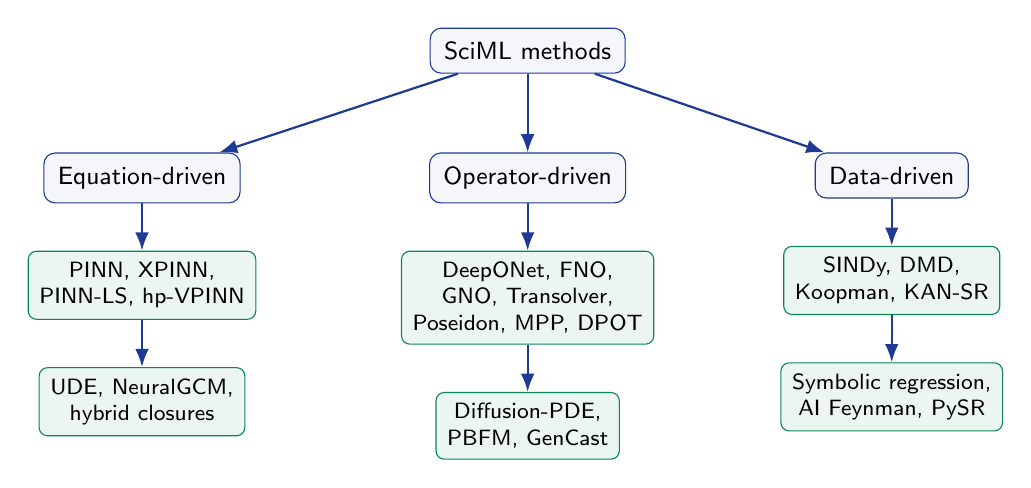
\begin{tikzpicture}[
    node/.style={draw=accent,fill=soft,rounded corners=4pt,inner sep=5pt,
                 align=center,font=\small\sffamily},
    leaf/.style={draw=accent3,fill=accent3!8,rounded corners=3pt,
                 inner sep=4pt,align=center,font=\footnotesize\sffamily},
    arrow/.style={-Latex,thick,accent}]
  \node[node] (root) {SciML methods};
  \node[node, below left=1cm and 2.4cm of root] (eq) {Equation-driven};
  \node[node, below=1cm of root] (op) {Operator-driven};
  \node[node, below right=1cm and 2.4cm of root] (data) {Data-driven};

  \draw[arrow] (root) -- (eq);
  \draw[arrow] (root) -- (op);
  \draw[arrow] (root) -- (data);

  \node[leaf, below=0.6cm of eq] (pinn) {PINN, XPINN,\\PINN-LS, hp-VPINN};
  \node[leaf, below=0.6cm of op] (no) {DeepONet, FNO,\\GNO, Transolver,\\Poseidon, MPP, DPOT};
  \node[leaf, below=0.6cm of data] (sindy) {SINDy, DMD,\\Koopman, KAN-SR};
  \node[leaf, below=0.6cm of pinn] (ude) {UDE, NeuralGCM,\\hybrid closures};
  \node[leaf, below=0.6cm of no] (gen) {Diffusion-PDE,\\PBFM, GenCast};
  \node[leaf, below=0.6cm of sindy] (sym) {Symbolic regression,\\AI Feynman, PySR};

  \draw[arrow] (eq) -- (pinn);
  \draw[arrow] (op) -- (no);
  \draw[arrow] (data) -- (sindy);
  \draw[arrow] (pinn) -- (ude);
  \draw[arrow] (no) -- (gen);
  \draw[arrow] (sindy) -- (sym);
\end{tikzpicture}
\end{center}


% =========================================================
\backmatter
\printbibliography[heading=bibintoc,title={References \& Further Reading}]

\end{document}
